\chapter{Kanban Setup \\
\small{\textit{-- Gavin Lam, Spurthi Setty, Annanya Jain, Luo Xu}}
\index{Kanban Setup} 
\index{Chapter!Kanban Setup}
\label{Chapter::Kanban Setup}}

For my DevOps project, I chose to use Atlassian JIRA to set up my Kanban board because I have some familiarity with it having used it once before in another class. \medskip

\noindent
First, I created a new project in Jira and selected the \textbf{Kanban template}. I decided to use the team-managed project option and gave it the name SSW 590 after the class. JIRA automatically provided the columns \textbf{To Do}, \textbf{In Progress}, and \textbf{Done}. \\


Step 1: Set up Jira Team 
\begin{center}
  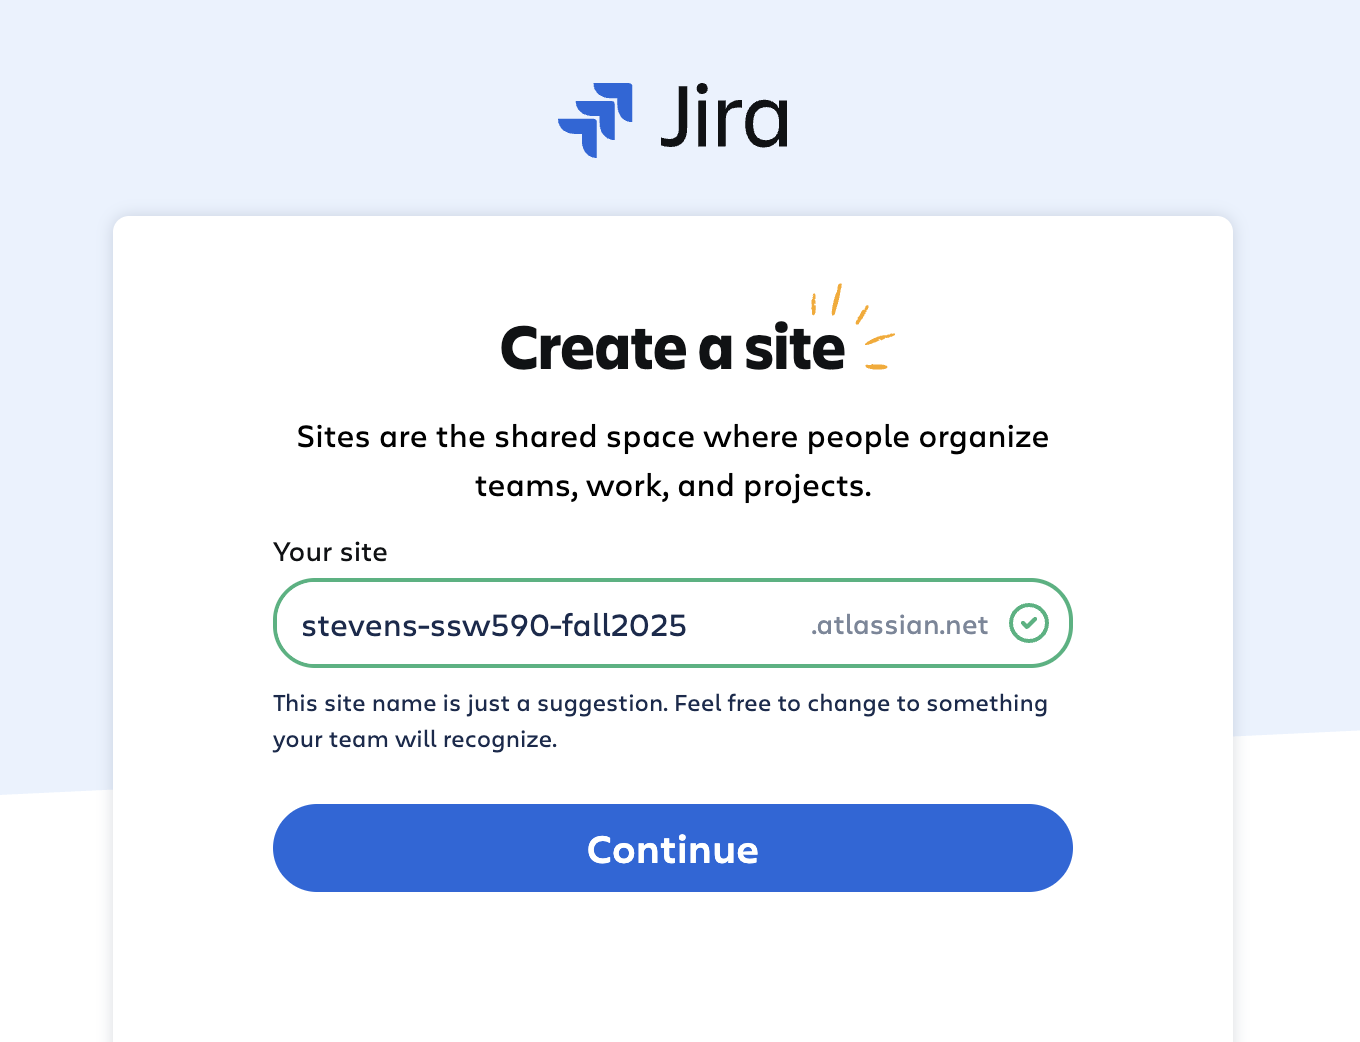
\includegraphics[width=0.7\textwidth]{png/Jira_team_setup.png}
\end{center}
I have chosen the name 'stevens-ssw590-fall2025' as the site name. \newpage

Step 2: Set up a Kanban Project 
\begin{center}
  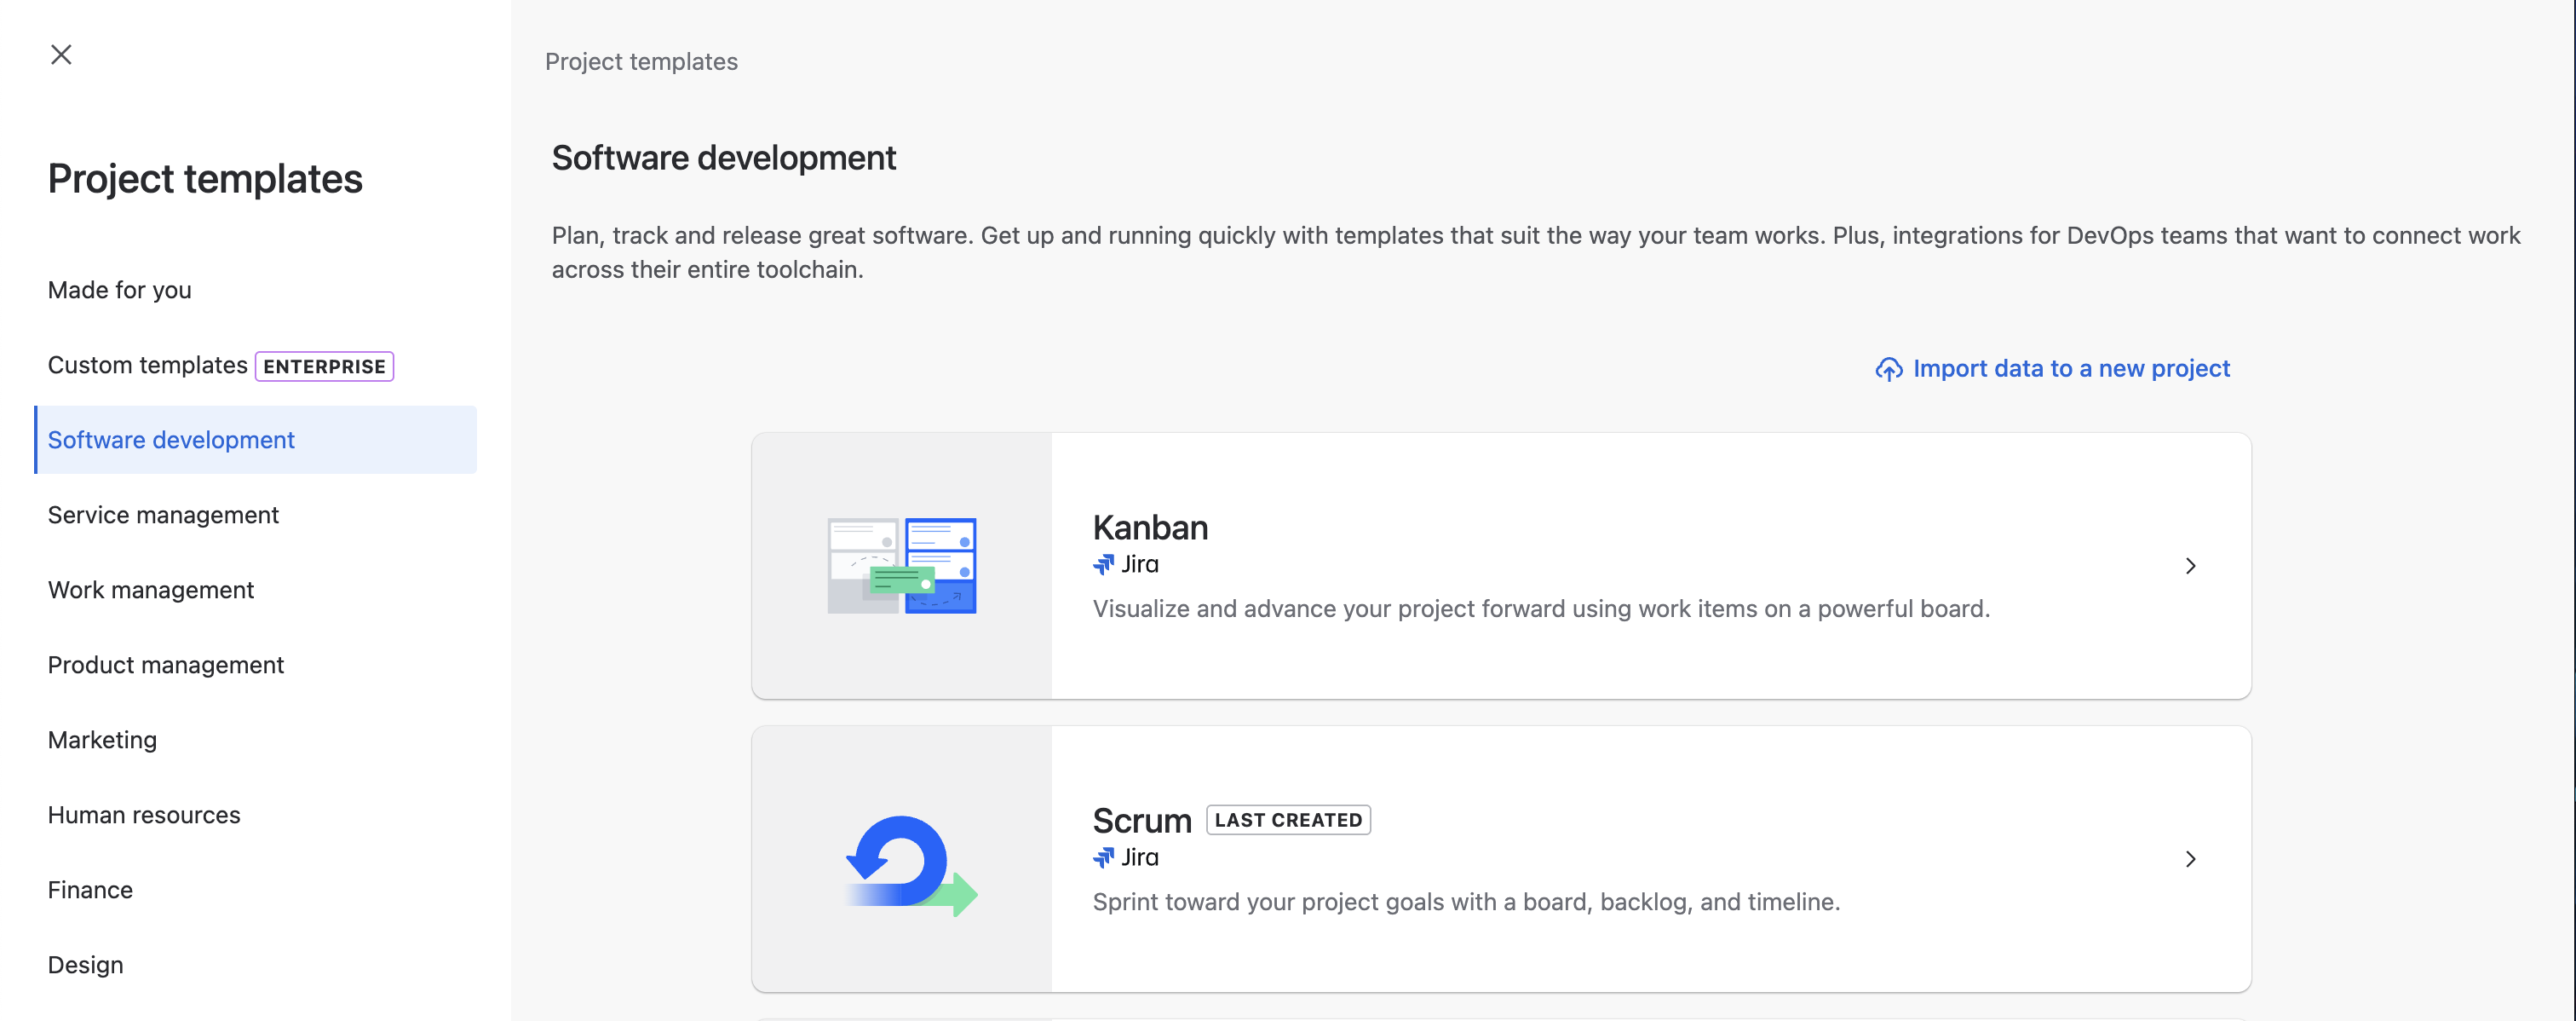
\includegraphics[width=0.9\textwidth]{png/creating_kanban_project2.png}
\end{center}

Step 3: Kanban
\begin{center}
  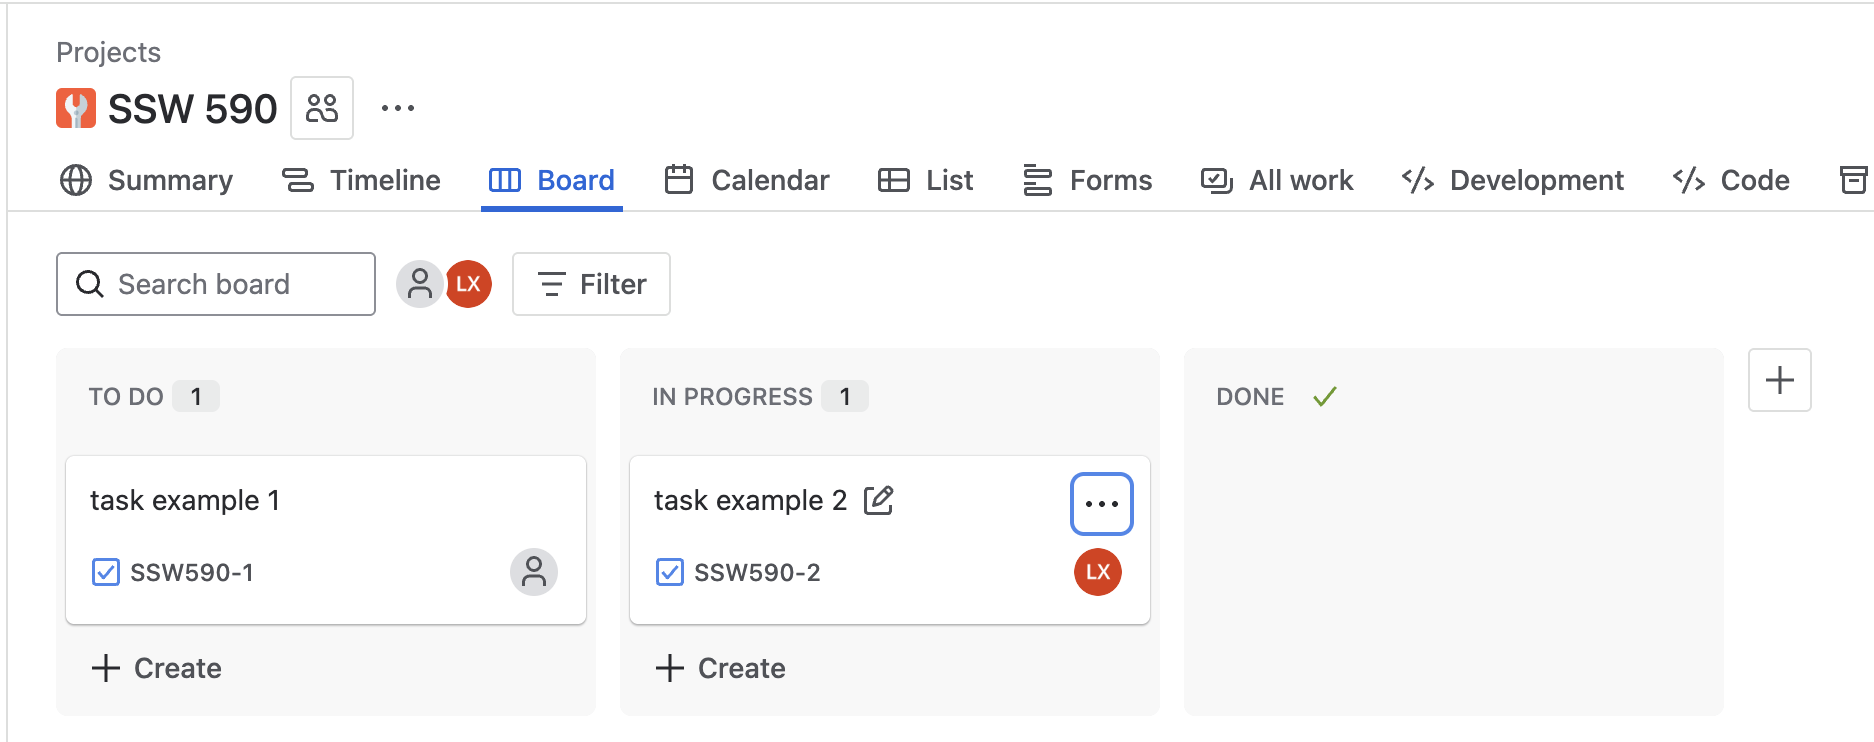
\includegraphics[width=0.9\textwidth]{png/kanban_example.png}
\end{center}